\documentclass[a4paper,8pt]{article}
\usepackage[utf8]{inputenc}
\usepackage[english]{babel} %language
\usepackage[
backend=biber,
style=alphabetic,
citestyle= authoryear
]{biblatex}
\usepackage{amssymb}
\usepackage{listings}
\usepackage{xcolor}
\usepackage{array}
\usepackage{float}

%CodeColours
\definecolor{codegreen}{rgb}{0,0.6,0}
\definecolor{codegray}{rgb}{0.5,0.5,0.5}
\definecolor{codepurple}{rgb}{0.58,0,0.82}
\definecolor{backcolour}{rgb}{0.95,0.95,0.92}
\definecolor{codeblue}{rgb}{0,0,0.80}

%Codestyle
\lstdefinestyle{mystyle}{
	backgroundcolor=\color{backcolour},   
	commentstyle=\color{codegreen},
	keywordstyle=\color{orange},
	numberstyle=\tiny\color{codegray},
	stringstyle=\color{codepurple},
	basicstyle=\ttfamily\footnotesize,
	identifierstyle=\color{codeblue},
	breakatwhitespace=false,         
	breaklines=true,                 
	captionpos=b,                    
	keepspaces=true,                 
	numbers=left,                    
	numbersep=5pt,                  
	showspaces=false,                
	showstringspaces=false,
	showtabs=false,                  
	tabsize=2,
	basicstyle=\scriptsize
}
%Set style
\lstset{style=mystyle}

%Images and similar
\usepackage{graphicx}
\graphicspath{.}

%timeline
\usepackage{tikz}
\usetikzlibrary{snakes}
\usepackage{rotating}

\title{Title}
\author{Simon dos Reis Spedsbjerg}

\newcommand{\Phases}{PHASES }
\newcommand{\phaseq}{PHASE1}

\usepackage{biblatex}

\begin{document}
	\maketitle
	
	\section{Problem}
	As data collection forever increases and systems ever becomes more depended on the quality of the data. Faulty data may damage the quality of analysis which is performed on the data, and outlier data may indicate another system is failing or an uncommon phenomenon has occurred on the sampled group.
	
	\section{Project}
	We intend to go into \Phases phases during this project.

	
	In the following, we see the expected timeline for the project.\newline
	%Timeline
	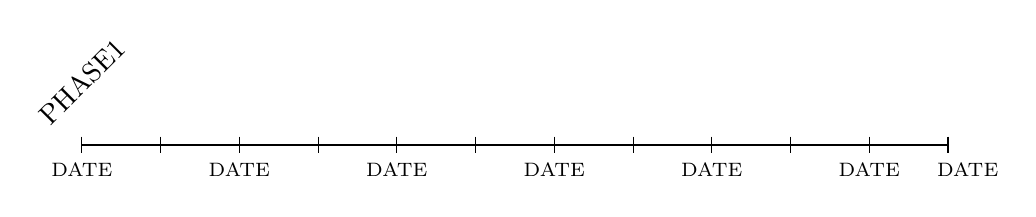
\begin{tikzpicture}
		%create the line
		\draw (-5,0) -- (6,0);
		
		%vertical lines
		\foreach \x in {-5, -4, -3, -2, -1, 0, 1, 2, 3, 4, 5, 6}
		\draw (\x cm, 3pt) -- (\x cm, -3pt);
		
		%draw
		\draw (-5,0) node[below=3pt] {\scriptsize DATE}; node[above=3pt] {$ $}; %start date
		
		\draw (-5,0)
		node[below=9pt] { }
		node[above=3pt] {\begin{turn}{45}\phaseq\end{turn}};
		
		\draw (-3,0)
		node[below=3pt] {\scriptsize DATE}
		node[above=3pt] {\begin{turn}{45}
				\phasew
		\end{turn}};
		
		\draw (-1,0)
		node[below=3pt] {\scriptsize DATE}
		node[above=3pt] {\begin{turn}{45}
				\phasee
		\end{turn}};
		
		\draw (1,0)
		node[below=3pt] {\scriptsize DATE}
		node[above=3pt] {\begin{turn}{45}
				\phaser
		\end{turn}};
		
		\draw (3,0)
		node[below=3pt] {\scriptsize DATE}
		node[above=3pt] {\begin{turn}{45}
				\phaset
		\end{turn}};
		
		\draw (5,0)
		node[below=3pt] {\scriptsize DATE}
		node[above=3pt] {\begin{turn}{45}
				\phasey
		\end{turn}};
		
		\draw (6.25,0) node[below=3pt] {\scriptsize DATE}; node[above=3pt] {$ $}; %end date
	\end{tikzpicture}
	
\end{document}